\section{Results}
\label{sec:results}
The galactic center and solar searches were preformed on 2628.1 days of SK-IV data, which corresponds to 161.9 kton-years.  The results of the searches are summarized in \cref{tab:results_low,tab:results_mid,tab:results_high}.  There are no indications of excesses from the galactic center or the sun.  The results are converted to event rate limits and presented in \cref{fig:evt_rate_limits}.  The locations of all events in the sky are shown in \cref{fig:skymap_zoomed,fig:skymap_all}.  As can be seen there is no visual clustering of events around the galactic center.


%\begin{table}


%\begin{adjustbox}{max width=\textwidth}
%	\begin{tabular}{lccccc}
%	\hline \hline
%	&  \parbox[t]{1.5cm}{ Expected\\ Bckg }& Data & \parbox[t]{1.5cm}{Signal\\ 90\% C.I.}  &  \parbox[t]{2cm}{Significance\\ of Excess}  &  \parbox[t]{4cm}{Significance of Excess \\ with trial factor}\\
 %\hline 
%	GC $5^\circ$ cone & $7.80 \pm 0.18$ &  7 & 0-4.8 & *** &*** \\
%	GC $10^\circ$ cone & $29.51 \pm 0.66$ &  24 & 0-5.0 & *** &*** \\
%	GC $15^\circ$ cone & $67.3 \pm 1.5$ &  70 & 0-17.7 &0.86$\sigma$&0.29$\sigma$\\
%	GC $20^\circ$ cone & $119.8 \pm 3.7$ &  127 & 0-27.2 &1.1$\sigma$& 0.48$\sigma$\\
%	GC $25^\circ$ cone & $189.2 \pm 4.2$ &  211 & 2.6-47.8 &1.8$\sigma$& 1.2$\sigma$\\
%	GC $30^\circ$ cone & $269.5 \pm 6.0$ &  292 & 0-53.5 &1.6$\sigma$& 0.96$\sigma$\\
%	GC $35^\circ$ cone & $364.8 \pm 8.1$ &  387 & 0-58.1 &1.4$\sigma$& 0.82$\sigma$\\
%	GC $40^\circ$ cone & $472.2 \pm 10.5$ &  502 & 0-71.8 &1.6$\sigma$& 0.93$\sigma$\\
%\hline
%	Sun $5^\circ$ cone & $7.87 \pm 0.12$ & 5 & 0-2.7 & ***&***\\
%\hline \hline
	
%	\end{tabular}
%	\end{adjustbox}
%	\caption{Results for low energy events}
%\label{tab:results_low}	
%\end{table}


\begin{table}
\resizebox{\linewidth}{!}{

	\begin{tabular}{lccc}
	\hline \hline
	& Expected Bckg& Data & Signal 90\% C.I.  \\
 \hline 
	GC $5^\circ$ cone & $8.6 \pm 0.7$ &  7 & 0-4.5 \\
	GC $10^\circ$ cone & $32.9 \pm 1.9$ &  24 & 0-3.7 \\
	GC $15^\circ$ cone & $74.4 \pm 3.6$ &  70 & 0-11.9 \\
	GC $20^\circ$ cone & $129.5 \pm 5.5$ &  127 & 0-19.5\\
	GC $25^\circ$ cone & $201.4 \pm 7.7$ &  211 & 0-37.5 \\
	GC $30^\circ$ cone & $290.3 \pm 10.2$ &  292 & 0-35.6\\
	GC $35^\circ$ cone & $394.1 \pm 13.0$ &  387 & 0-33.1\\
	GC $40^\circ$ cone & $511.2 \pm 16.0$ &  502 & 0-37.6\\
\hline
	Sun $5^\circ$ cone & $7.74 \pm 0.19$ & 5 & 0-2.8 \\
\hline \hline
	
	\end{tabular}
}

	\caption{Results for low energy events}
\label{tab:results_low}	
\end{table}


\begin{table}
\resizebox{\textwidth}{!}{
	\begin{tabular}{lccccc}
	\hline \hline
	&  Expected Bckg & Data & Signal 90\% C.I.  \\
	\hline 
	GC $5^\circ$ cone &$1.6\pm0.3$&1&0-2.9 \\
	GC $10^\circ$ cone &$6.3\pm0.84$&4&0-3.0 \\
	GC $15^\circ$ cone & $13.9\pm1.6$&12&0-5.7\\
	GC $20^\circ$ cone &$23.9\pm2.4$&19&0-5.2\\
	GC $25^\circ$ cone & $36.4\pm3.3$&31&0-7.2\\
	GC $30^\circ$ cone & $50.6\pm4.3$&50&0-14.3\\
	GC $35^\circ$ cone &$69.7\pm5.5$&70&0-17.7\\
	GC $40^\circ$ cone & $92.1\pm6.9$&94&0-22.4\\
\hline
	Sun $5^\circ$ cone &$1.29 \pm 0.08$ &1& 0-3.1\\
\hline \hline
	
	\end{tabular}	
} 
	\caption{Results for medium energy events}
\label{tab:results_mid}	
	\end{table}


\begin{table}
\resizebox{\textwidth}{!}{

	\begin{tabular}{lccccc}
	\hline \hline
	&  Expected Bckg  & Data &Signal 90\% C.I.  \\
	\hline 
	GC $5^\circ$ cone &$0.011\pm0.003$ & 0&0-2.5 \\
	GC $10^\circ$ cone & $0.041\pm0.012$ & 0&0-2.4\\
	GC $15^\circ$ cone & $0.096\pm0.029$ & 0&0-2.4\\
	GC $20^\circ$ cone & $0.17\pm0.05$ & 0&0-2.3\\
	GC $25^\circ$ cone & $0.26\pm0.08$ & 0&0-2.2\\
	GC $30^\circ$ cone & $0.37\pm0.11$ & 0&0-2.1\\
	GC $35^\circ$ cone & $0.49\pm0.15$ & 0&0-2.0\\
	GC $40^\circ$ cone &$0.63\pm0.19$ & 0&0-1.9\\
\hline
	Sun $5^\circ$ & $0.011\pm 0.003$ & 0 & 0-2.5\\
\hline \hline
	
	\end{tabular}

} 
		\caption{Results for high energy events}
\label{tab:results_high}	
	
\end{table}	

\begin{figure}
	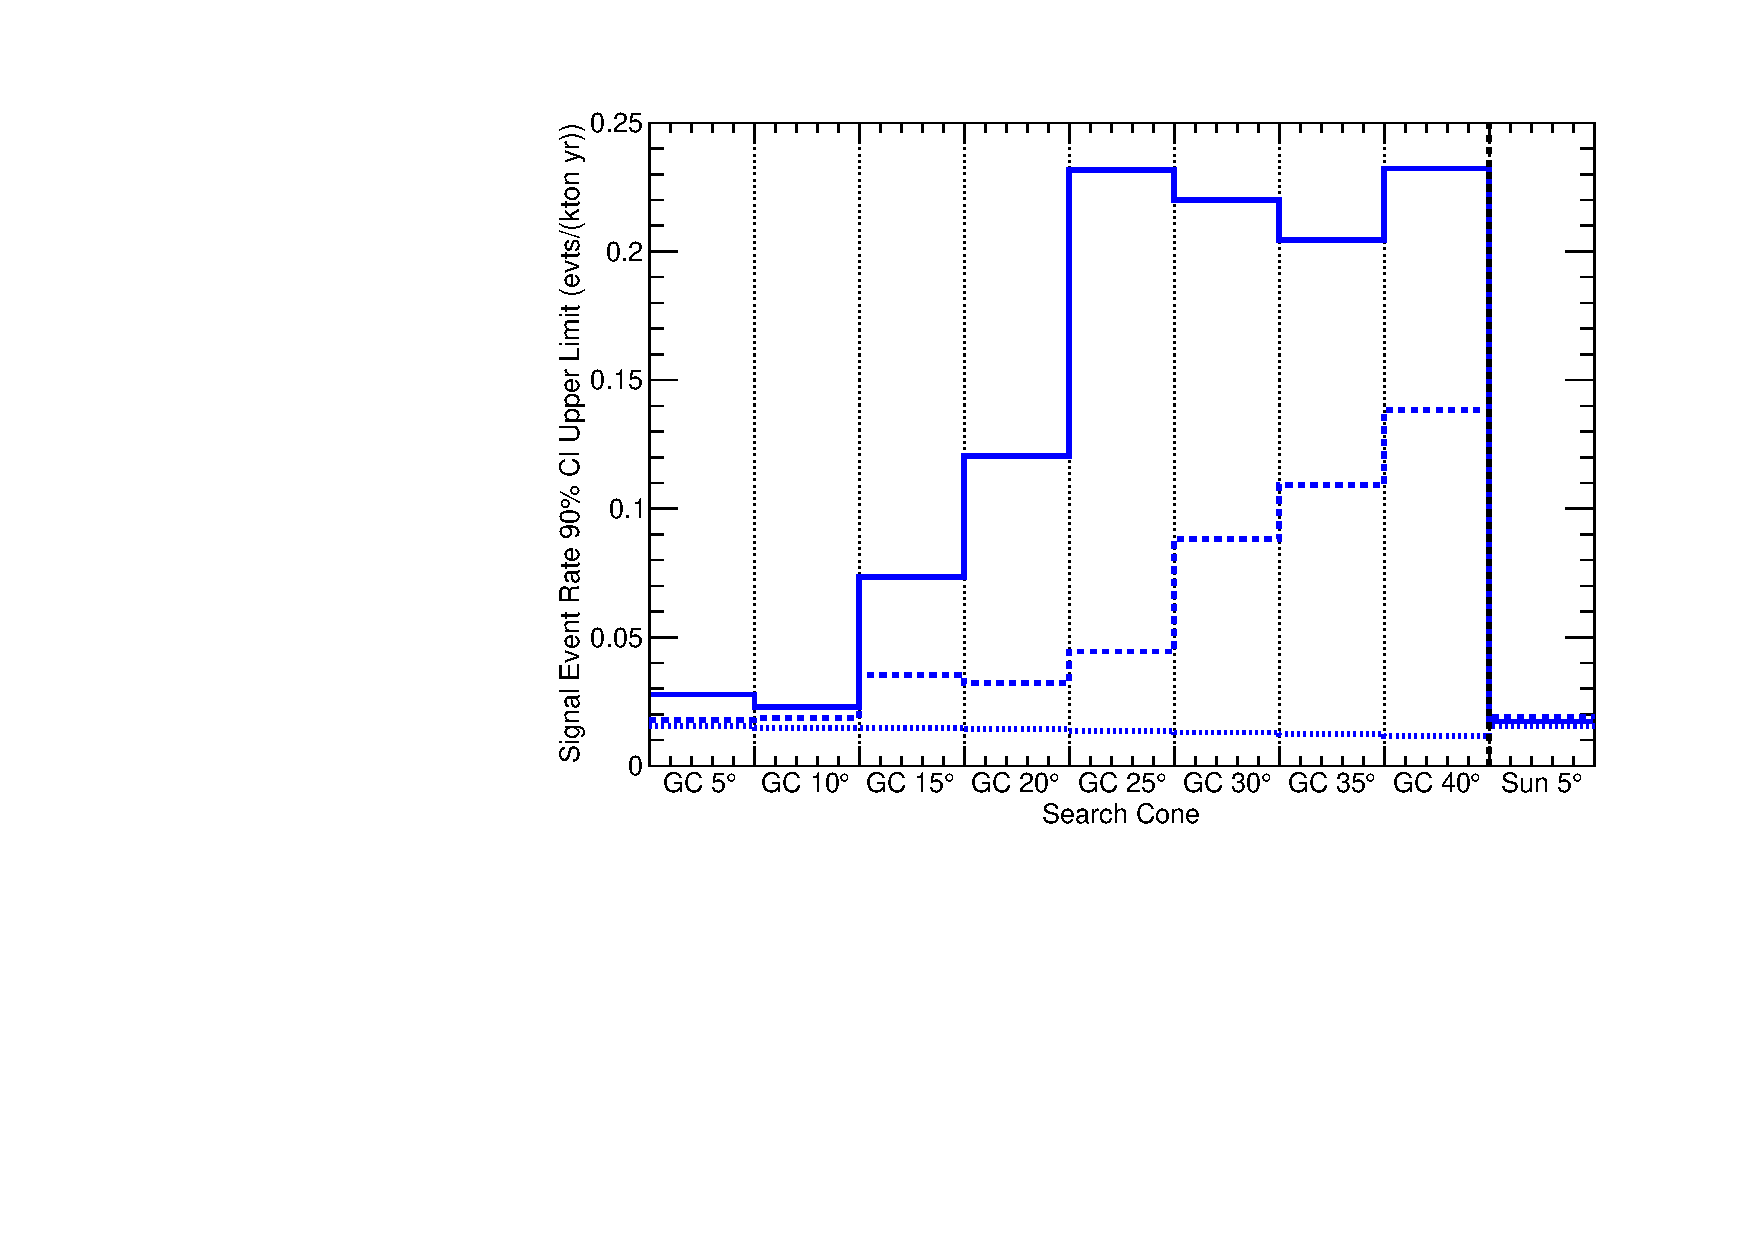
\includegraphics[width=0.8\textwidth]{figures/evt_rate_limits.pdf}
	\caption{Signal event rate 90\% C.I. upper limits for SubGeV (solid line), Mid Energy (dashed line), and High Energy (dotted line) samples.}
	\label{fig:evt_rate_limits}

\end{figure}


\begin{figure}
	\centering
	\subfigure[Low Energy]{	
	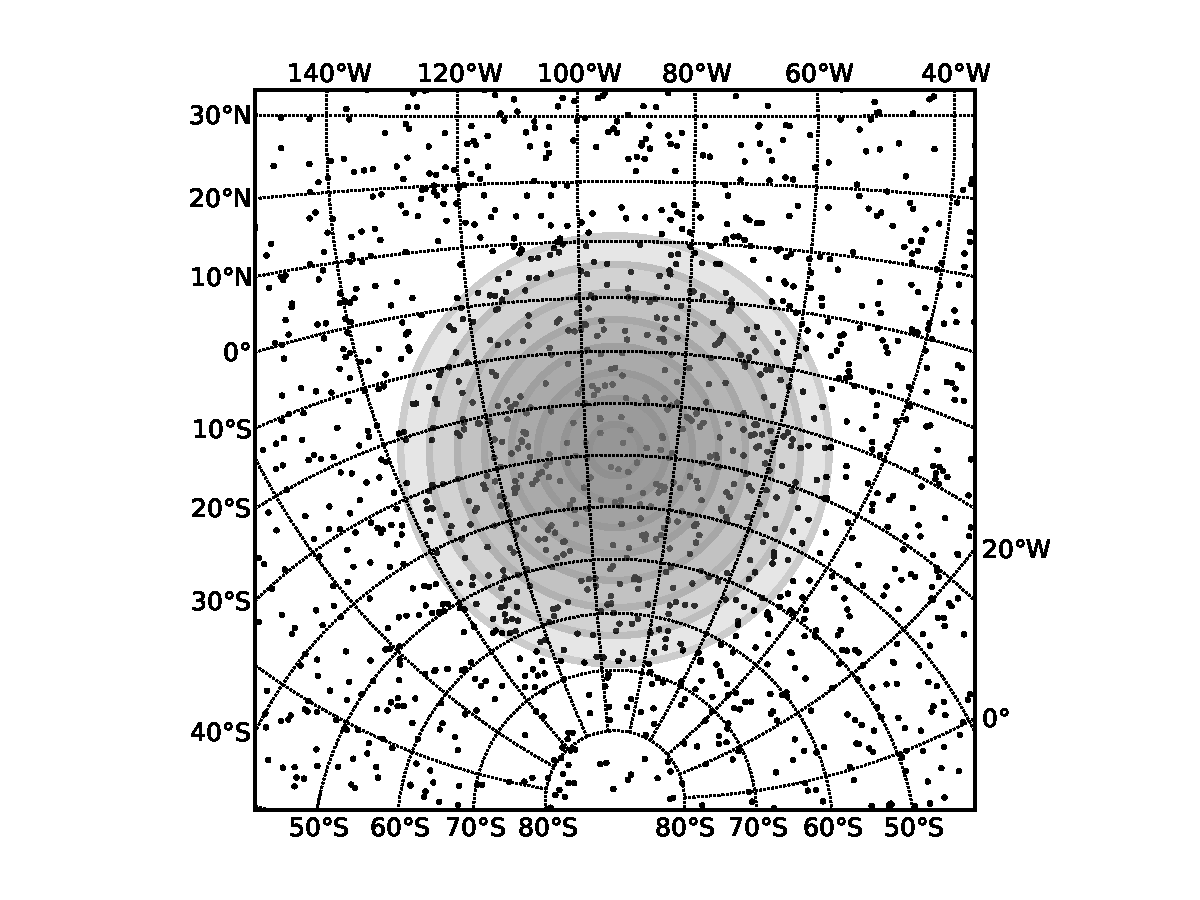
\includegraphics[width=0.3\textwidth]{figures/sky_map_zoomed_low.pdf}
	\label{fig:skymap_zoomed_low}
	}
	\subfigure[Mid Energy]{
	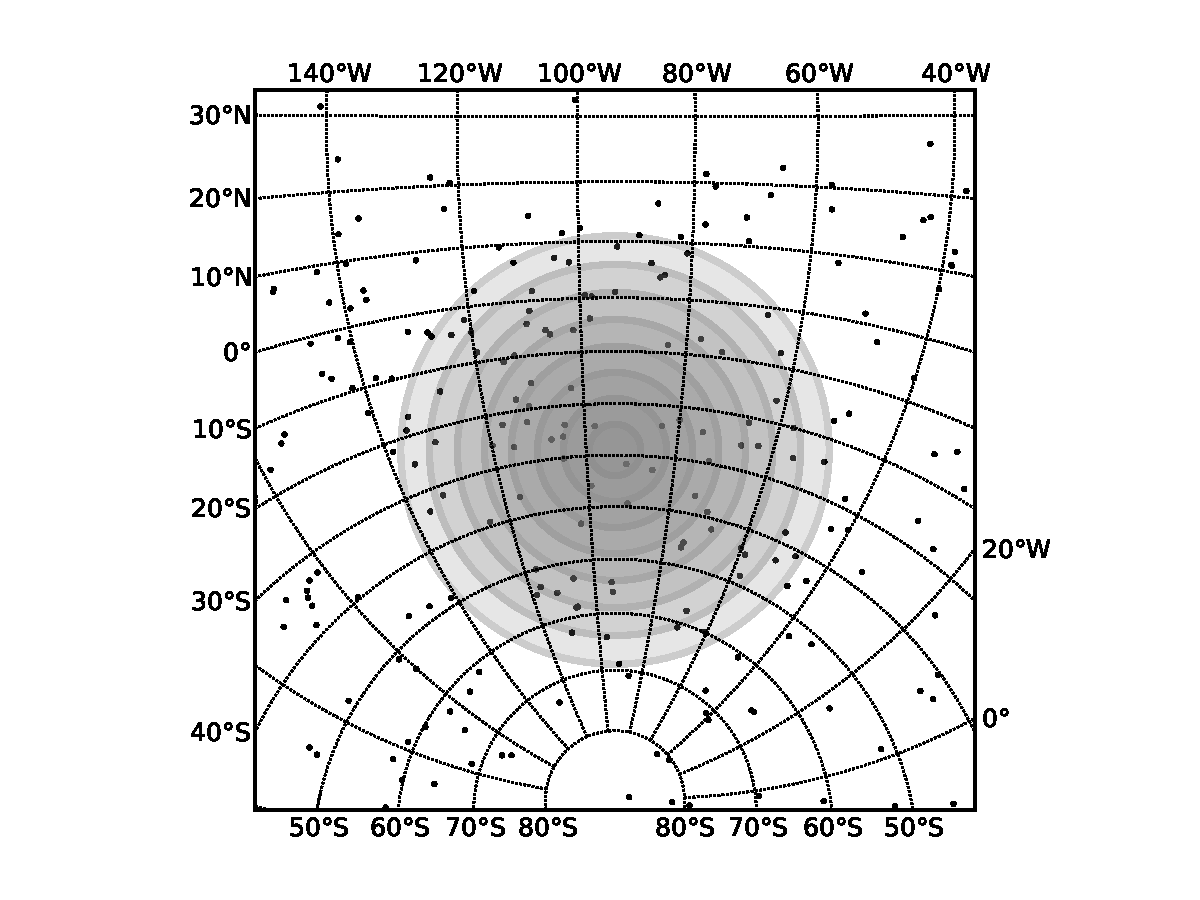
\includegraphics[width=0.3\textwidth]{figures/sky_map_zoomed_mid.pdf}
	\label{fig:skymap_zoomed_mid}
	}	
	\subfigure[Mid Energy]{
	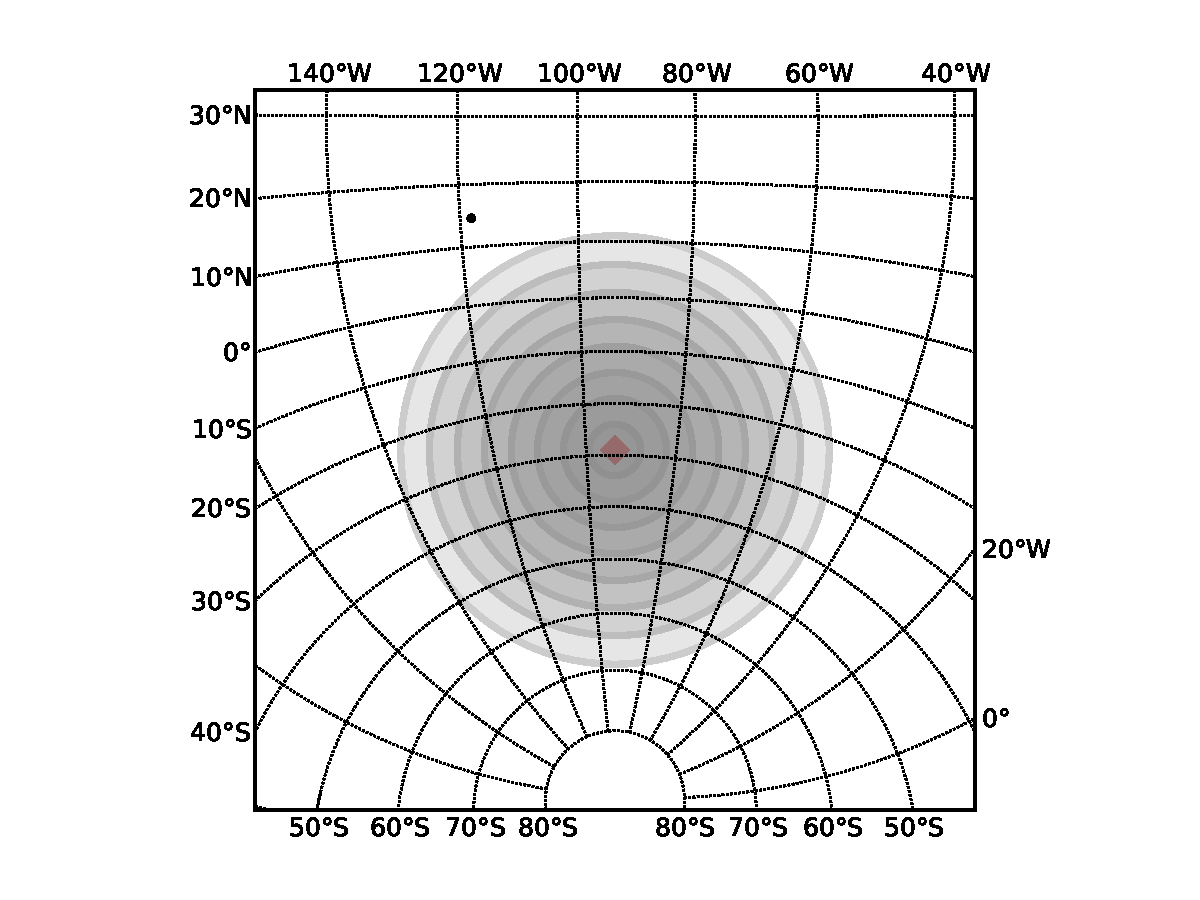
\includegraphics[width=0.3\textwidth]{figures/sky_map_zoomed_high.pdf}
	\label{fig:skymap_zoomed_high}
	}
	\caption{Location of all events passing analysis cuts near the galactic center.  The 8 grey circles show the 8 cones around the galactic center used in the analysis.}
	\label{fig:skymap_zoomed}
\end{figure}

\begin{figure}
	\centering
	\subfigure[Low Energy]{	
	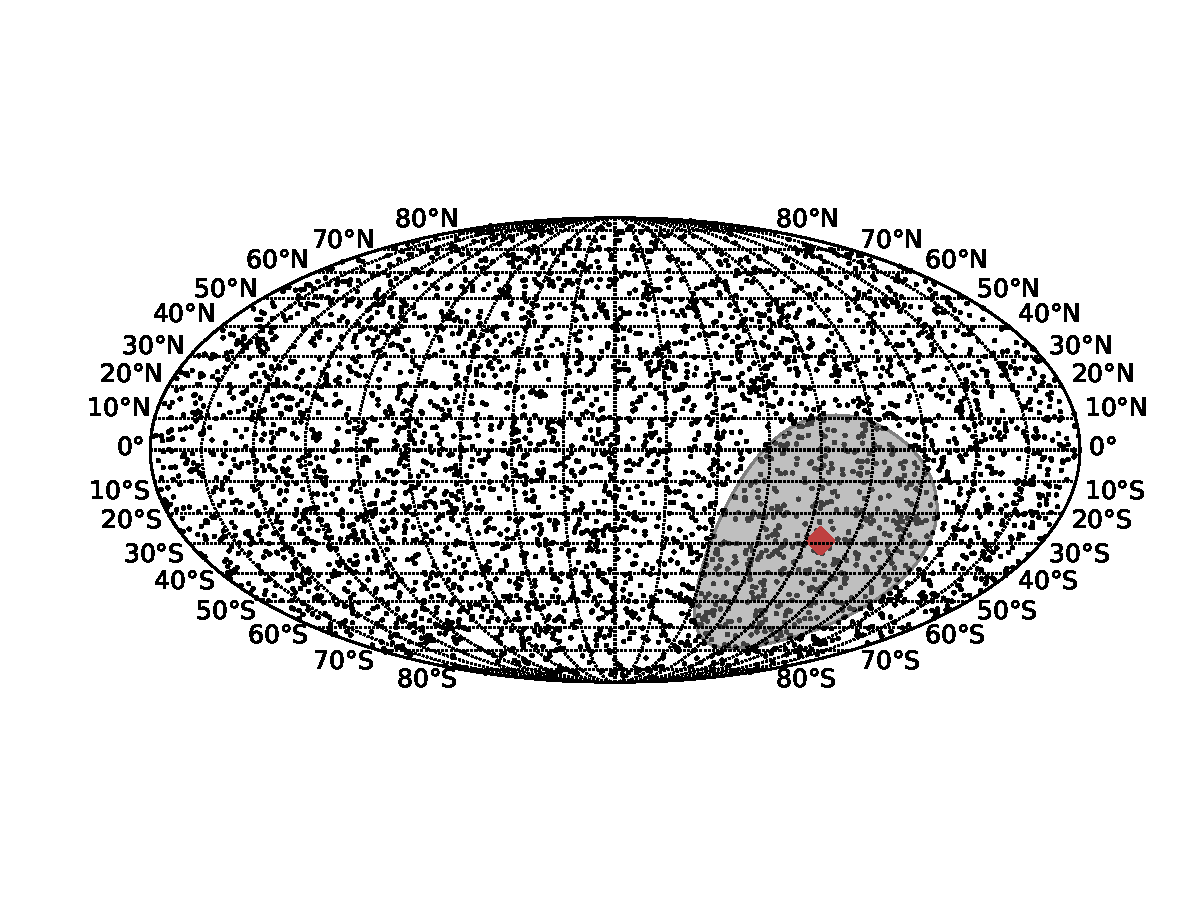
\includegraphics[width=0.3\textwidth]{figures/sky_map_all_events_low.pdf}
	\label{fig:skymap_all_low}
	}
	\subfigure[Mid Energy]{
	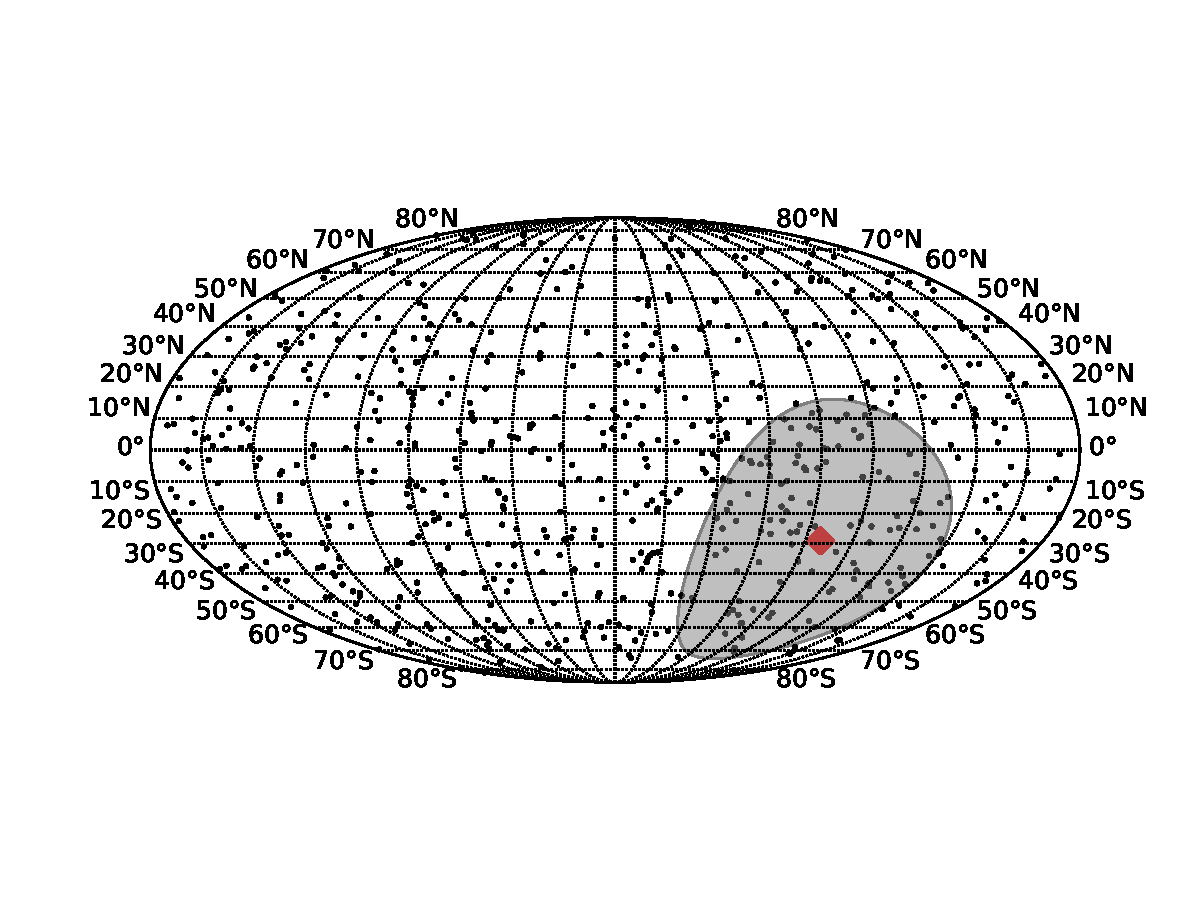
\includegraphics[width=0.3\textwidth]{figures/sky_map_all_events_mid.pdf}
	\label{fig:skymap_all_mid}
	}	
	\subfigure[Mid Energy]{
	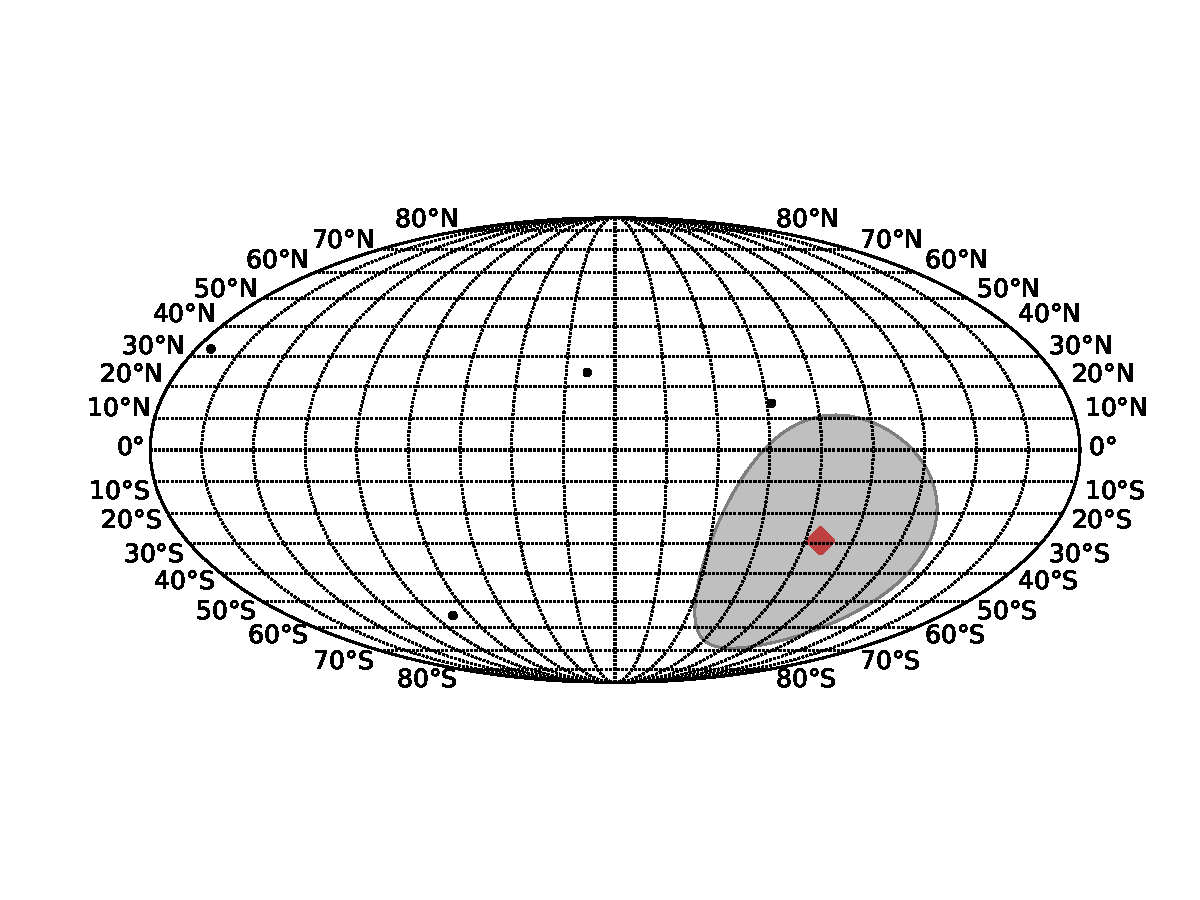
\includegraphics[width=0.3\textwidth]{figures/sky_map_all_events_high.pdf}
	\label{fig:skymap_all_high}
	}
	\caption{Location of all events passing analysis cuts.  The grey shows a 40$^\circ$ cone around the galactic center, which is shown by the red diamond}
	\label{fig:skymap_all}
\end{figure}

Limits were also calculated on a simple model, as described in \cref{sec:limits_simple_model}.  Since the point with $\sigma_\textrm{tot}$ is allowed at 90\% CI, the 90\% CI contours can be interpreted as 90\% CI upper limits.  These upper limits are presented for $m_{\gamma '}=20 MeV$ in \cref{fig:limits_on_model}.  When $E_\textrm{max}>10$ GeV, the effect of the detector energy threshold is negligable, and the 90\% CI upper limit on $\sigma_{\textrm{tot}}/m_A^2$ remains constant as $E_\textrm{max}$ increases.  In this region the limit for $m_{\gamma '}=20 MeV$ with the NFW halo model is found to be $1.5 \times 10^{-37}$(cm$^2$/GeV$^2$).

\begin{figure}
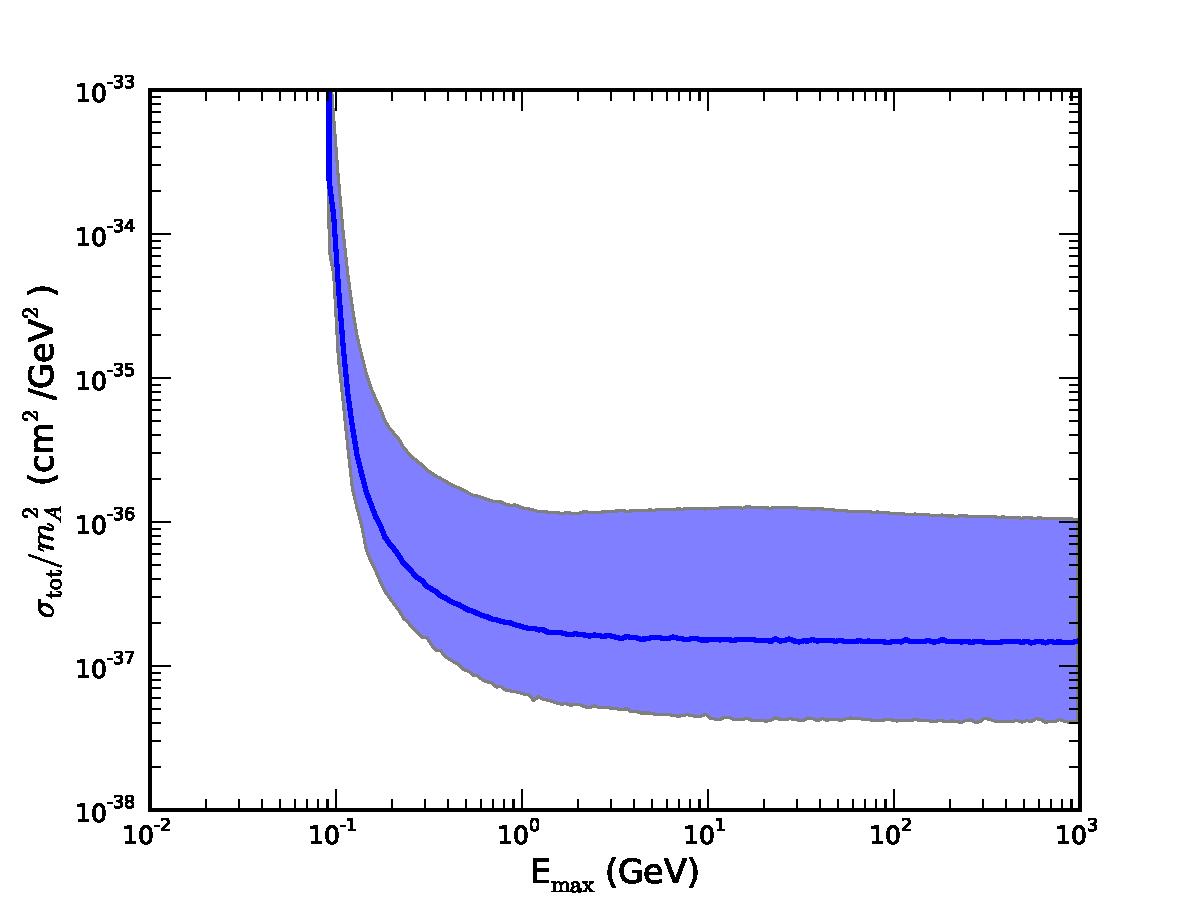
\includegraphics[width=0.8\textwidth]{figures/limits_mg_20MeV_toymc_new.pdf}
\caption{Limits on simple model, for $m_{\gamma '}=20$ MeV.  The dark blue line is for the NFW halo, and the upper and lower limits of the band are for the Kravtsov and Moore models, respectively.}
\label{fig:limits_on_model}
\end{figure}

